\section{Vorgehen}
In dem Versuch werden mit verschiedenen Gastemperaturen, die entstehenden Druckänderungen bei Volumenveränderung gemessen. Hier für wird, wie in Abbildung \ref{fig:Aufbau} dargestellt, das Gas in einer Glasküvette, umgeben von einem von einem Thermostat auf konstanter Temperatur gehaltenes Wärmebad, erwärmt. Das Thermometer dient zur Kontrolle der Temperatur, da diese (wahrscheinlich durch Abkühlen in den Zuleitungen) abweicht, sodass die Temperatureinstellung im Thermostat entsprechend angepasst werden kann.\\
 Mithilfe des Handrades wird nun Quecksilber, welches nahezu inkompressibel ist, nach oben gedrückt und somit das für das Gas zur Verfügung stehendes Volumen verkleinert bzw. vergrößert. Jede $\unit[0.25]{cm^3}$ bzw. $\unit[0.1]{cm^3}$ ab $V<\unit[1.5]{cm^3}$ sowie bei der Messreihe mit überkritischer Temperatur, wird der resultierende Druck $[\mathrm{100kPa}]$ am Manometer abgelesen. Die Messung wird jeweils zweimal durchgeführt, einmal für eine Volumenverkleinerung und einmal für eine Volumenvergrößerung.\\
Die Messungen für insgesamt neun Temperaturen wird auf drei Gruppen aufgeteilt, die Ergebnisse anschließen untereinander aufgeteilt


\begin{figure}
\begin{center}
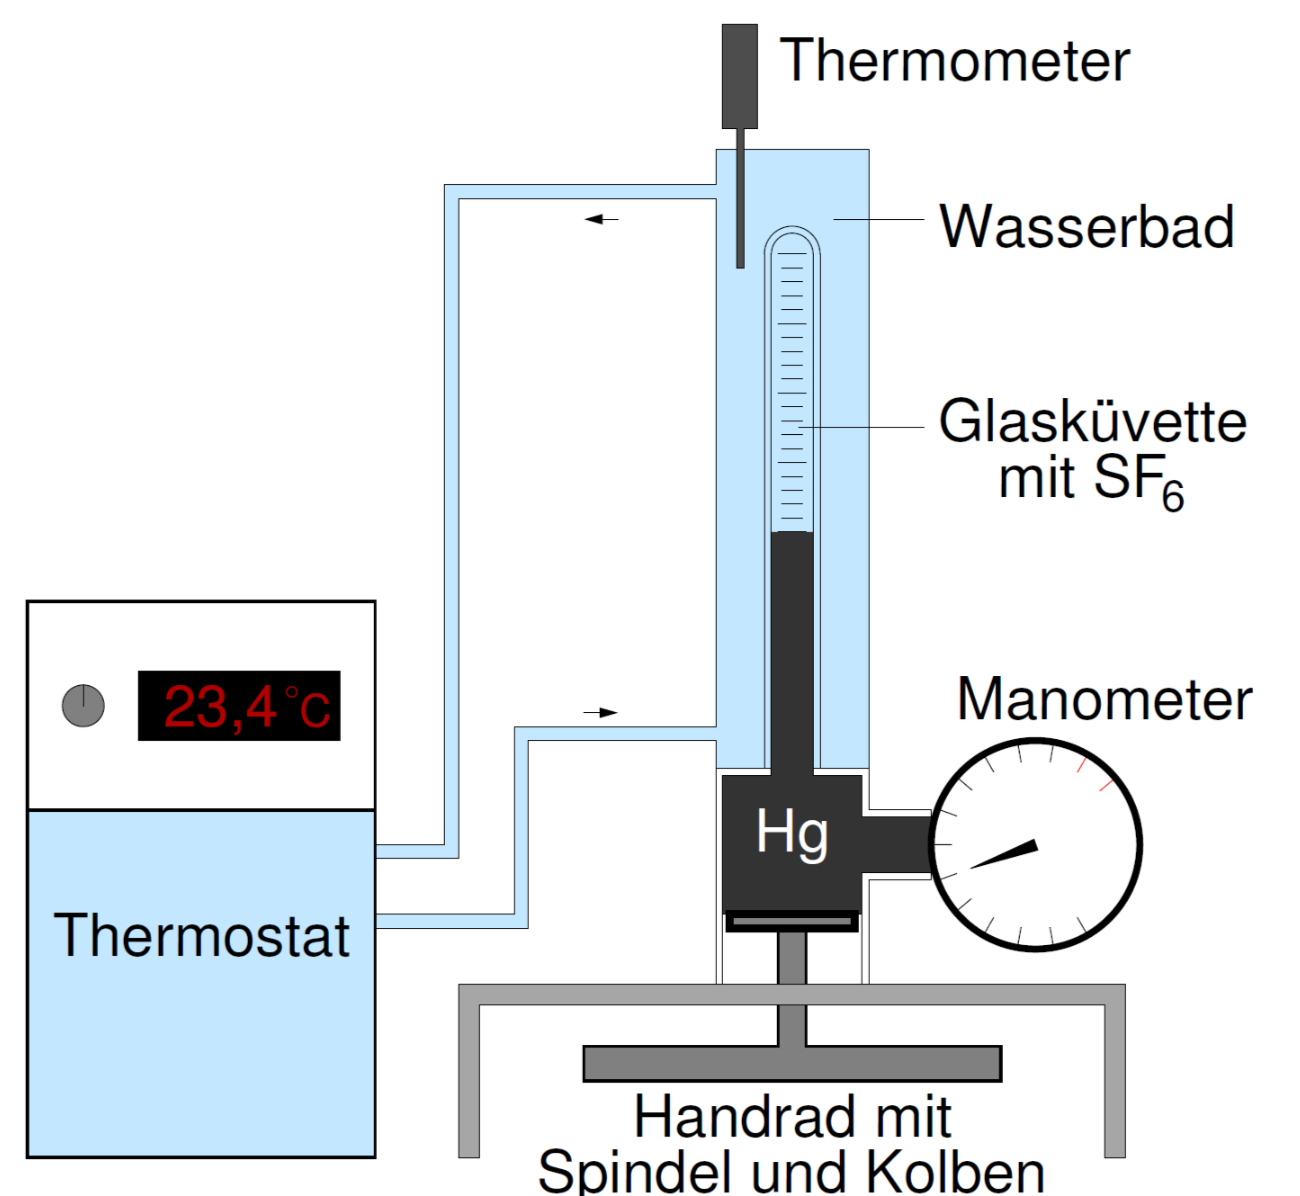
\includegraphics[width=0.5\textwidth]{Bilder/Versuchsaufbau.png}
\caption{Versuchsaufbau}
\label{fig:Aufbau}
\end{center}
\end{figure}